\documentclass[11pt,a4paper]{article}
\usepackage[T1]{fontenc}
\usepackage[left=2cm, right=2cm, top=2cm, bottom=2cm]{geometry}
\usepackage{graphicx}
\usepackage{mathtools}
\usepackage{amssymb}
\usepackage{amsthm}
\usepackage{amsfonts}
\usepackage{thmtools}
\usepackage{xcolor}
\usepackage{nameref}
\usepackage[colorlinks=true, linkcolor=black, urlcolor=black, citecolor=black]{hyperref}

\usepackage{physics}
\usepackage{amsmath}
\usepackage{tikz}
\usepackage{mathdots}
\usepackage{yhmath}
\usepackage{cancel}
\usepackage{color}
\usepackage{siunitx}
\usepackage{array}
\usepackage{multirow}
\usepackage{dsfont}

\usepackage{amssymb}
\usepackage{gensymb}
\usepackage{tabularx}
\usepackage{extarrows}
\usepackage{booktabs}
\usetikzlibrary{fadings}
\usetikzlibrary{patterns}
\usetikzlibrary{shadows.blur}
\usetikzlibrary{shapes}

\usepackage{placeins}




\theoremstyle{definition}
\newtheorem{defn}{Definition}


\title{MonteCarlo Integration}
\author{Ali Fele Paranj}

\newtheoremstyle{Example}
{\topsep}   % Space above
{\topsep}   % Space below
{}  % Body font
{}          % Indent amount
{\bfseries} % Theorem head font (bold)
{.}         % Punctuation after theorem head
{ }         % Space after theorem head
{}          % Theorem head spec


\theoremstyle{Example}
\newtheorem{example}{Example}



\newcommand{\Prob}{\mathbb{P}}
\newcommand{\set}[1]{\{#1\}}
\newcommand{\N}{\mathbb{N}}
\newcommand{\R}{\mathbb{R}}
\newcommand{\E}{\mathbb{E}}



\begin{document}
	\maketitle
	\begin{abstract}
		Monte Carlo integration method is discussed.
	\end{abstract}
	
	\section{Introduction}
	Let $ (\Omega=[0,1],\mathcal{F},\Prob) $ be a probability space, with $ \mu $ as the probability density function for the space, i.e. $\mu = d\Prob/dx $. So for $ A \in \mathcal{F} $ we have
	\[  \Prob(A) = \int_\Omega \mathds{1}_A d\Prob = \int_\Omega \mathds{1}_A \mu(x) dx = \int_A \mu(x)dx. \]
	Assuming that we know $ \mu(x) $, calculating $ \Prob(A) $ can be done by calculating the specified integral, which can be approximated by integral approximation methods. However, in reality, the domain of integration might be very large, or we might not be able to evaluate $ \mu(x) $ because of a complicated normalization constants. So it might be difficult to calculate the RHS integral. Here, we will demonstrate the Monte Carlo method to evaluate the integral.
	
	Let $ (Y_i)_{i\in\N} $ be a sequence of i.i.d. random variables with $ Y_n \sim \mu $. Define
	\[ Z_n = \frac{\sum_{i=1}^n \mathds{1}_{Y_i\in A}}{n}. \]
	Using the law of large numbers, we know that
	\[ Z_n \to \E[\mathds{1}_{Y_1\in A}]  \]
	in probability as $ n\to\infty $. Observe that $ \E[\mathds{1}_{Y_1\in A}] = \Prob(Y_1\in A) = \mu(A) $. So
	\[ Z_n \to \mu(A) = \int_A\mu(x)dx \qquad \text{as $ n\to \infty $}, \]
	where the convergence is in probability. And by the central limit theorem 
	\[ \operatorname{Var}(Z_n) \propto \frac{1}{n}. \]
	
	\begin{example}
		Let $ \mu $ be the uniform distribution on the interval $ [0,1] $, (i.e. Lebesgue measure). This distribution will be very important in the following sections. Let $ A = [0.23,0.65] $. To calculate $ \mu(A) $ (which a prior we know $ \mu(A) = 0.42 $), let $ (Y_i)_{i\in\N} $ be i.i.d. with $ Y_i \sim \operatorname{Uniform}(0,1) $. Define
		\[ Z_n = \frac{\sum_{i=1}^n \mathds{1}_{Y_i\in A}}{n}. \] 
		Note that the interpretation of $ Z_n $ in a computer program is ``generate $ n $ uniform random numbers in $ [0,1] $ and count how many of them fall in $ A $, divide by $ n $''. So if you generate a long string of random values $ (w_0,w_1,w_2,\cdots) $, we perform a rolling average of number of values that fall in $ A $. The dependence on $ \omega $, is when we have another realizations. The following figure demonstrates $ Z_n $ vs $ n $ over different realizations (i.e. different curves corresponds to different $ \omega \in \Omega_\text{comp} $. In reality, in computer $ \Omega_\text{comp} = \set{0,1}^\N $ and all of the real-valued random numbers are approximated to certain number of bits).
		
		\begin{figure}
			\centering
			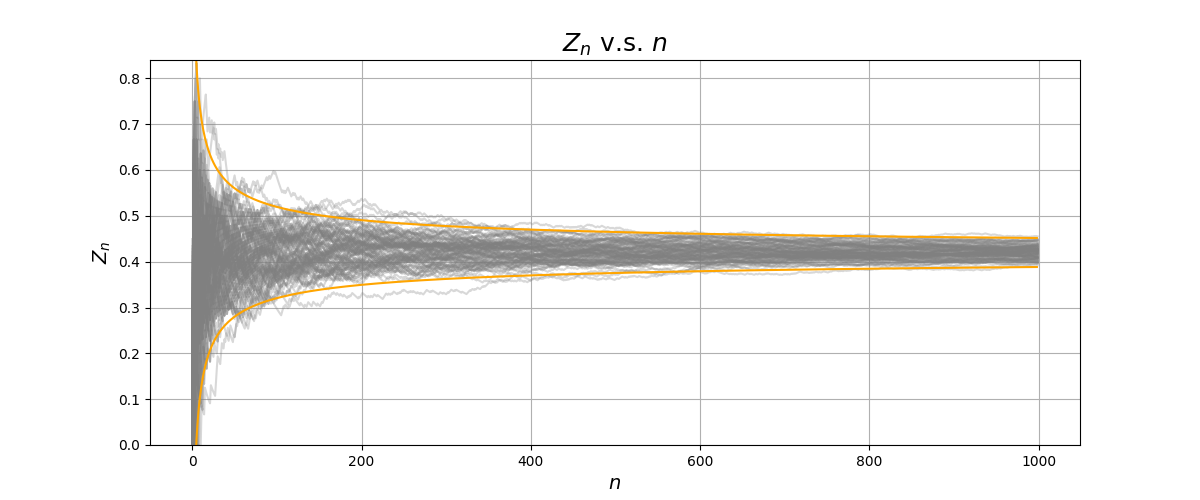
\includegraphics[width=0.7\linewidth]{ZnVsn}

			\label{fig:znvsn}
		\end{figure}
		
	\end{example}
	
	
	
	
	\section{In reality}
	In reality, we often start with a function that we want to integrate, 
	
	
	
	
	
	\section{Playground}
	
	Let $ (\Omega,\mathcal{F},\Prob) $ be any probability space, and let $ A \in \mathcal{F} $. We are interested in calculating $ \Prob(A) $. At first, this question might seem like a trivial question, as when we say we have a probability space $ (\Omega, \mathcal{F},\Prob) $ we are already specifying all necessary information to know $ \Prob(A) $. However, Assume that $ \Prob(A) $ is unknown to us and we want to see if there are any methods that we can use to approximate it to arbitrary precision. for instance, assume that we have our computer in our disposal, where we have access to the probability space $ \set{0,1}^\N $ with the probability that the cylinder sets $ A_{w_0,\cdots,w_n} $ has probability $ 1/2^n $. Or equivalently, we have access to a fair coin the can generate $ 0 $ or $ 1 $ with equal probability. Or equivalently, we have access to i.i.d. random variables $ (Z_i)_i $ with distribution $ \mu $. For instance, w
	
	
	

\end{document}

